\section{Results}

\begin{frame}
\frametitle{Overview of results}
\begin{itemize}
\item Results for tridiagonal solver (NEATO)
\begin{itemize}
    \item Global memory v/s shared memory implementations
    \item Compared against library solvers
        (multicore CPU and GPU)
\end{itemize}
\item Results for compact finite difference application
\begin{itemize}
    \item Profiling results
    \item Scaling results
    \item Comparison with CPU-only approach
\end{itemize}
\end{itemize}
\end{frame}

\begin{frame}
\frametitle{Global memory v/s shared memory implementations}
\footnotesize
\begin{columns}
\begin{column}{0.5\textwidth}

\begin{block}{Benchmark details}
\begin{itemize}
\item Solving multiple tridiagonal systems on single GPU
\item Up to $2048$ equations in $2048$ variables (2-D)
    and $512^2$ equations in $512$ variables (3-D)
\item GPU: NVIDIA Tesla K20
\end{itemize}
\end{block}

\begin{itemize}
\item For 2-D problems, shared memory clearly better
\item For 3-D problems, shared memory speedup
    is smaller
\item Thread inactivity in shared memory leads
    to reduced performance
\end{itemize}
\end{column}
\begin{column}{0.5\textwidth}
\centering
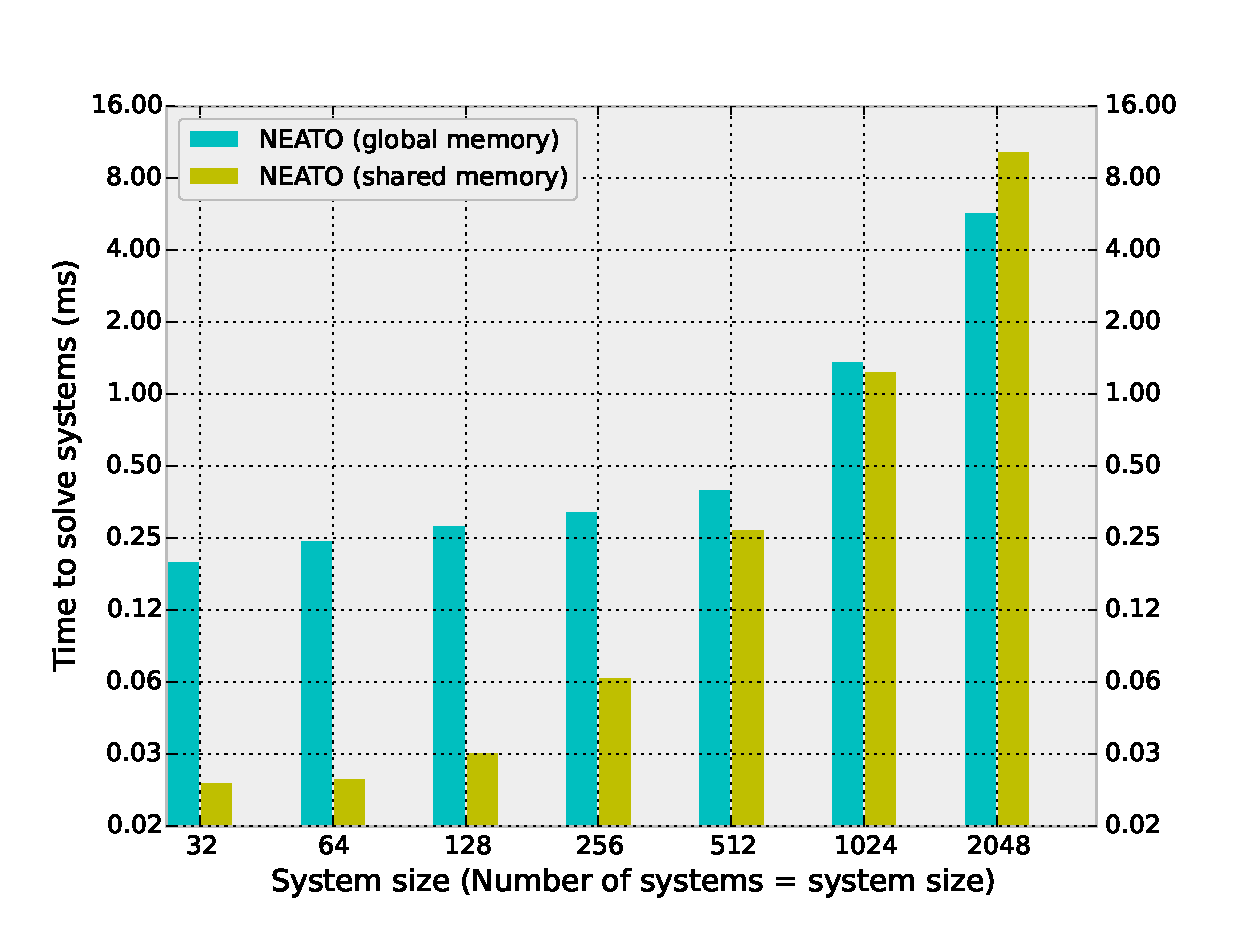
\includegraphics[width=140px]{img/global-vs-shared-2d.eps}

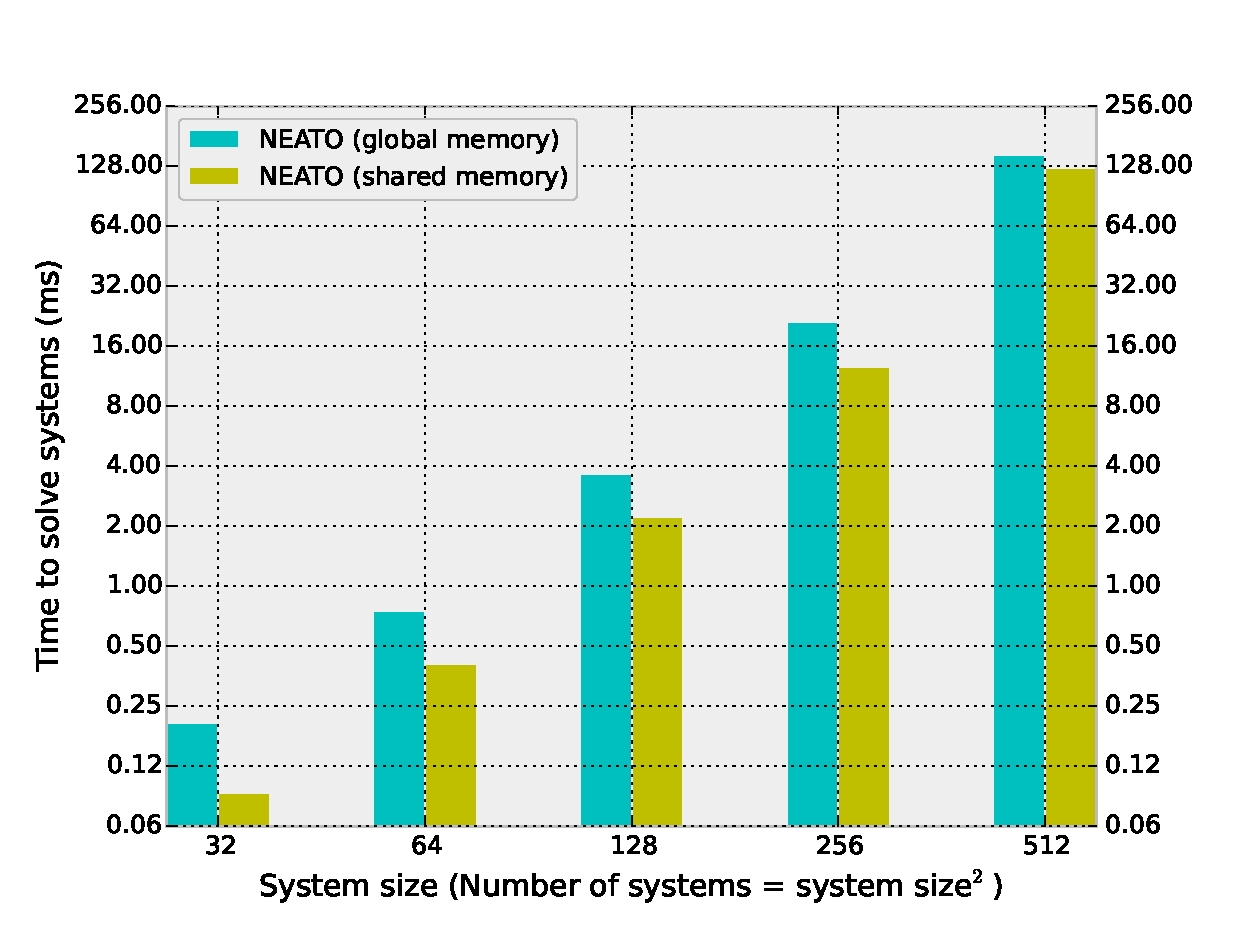
\includegraphics[width=140px]{img/global-vs-shared-3d.eps}
\end{column}
\end{columns}
\end{frame}

\begin{frame}{Comparison with library solvers}
\footnotesize
\begin{block}{Benchmark details}
\begin{itemize}
\item Solving multiple tridiagonal systems on single GPU and multicore CPU
\item Up to $2048$ equations in $2048$ variables (2-D)
    and $512^2$ equations in $512$ variables (3-D)
\item GPU: NVIDIA Tesla K20
\item CPU: Intel Xeon E5 v2
\item Do \emph{not} include cost of CPU-GPU transfer
\item Library solver details:
\begin{itemize}
    \footnotesize
    \item Intel MKL \texttt{dgtsv} (Gaussian elimination with partial pivoting)
    \item CUSPARSE \texttt{dgtsv} (Hybrid CR+PCR)
\end{itemize}
\item \texttt{-02} level compiler optimizations
\item Double precision
\end{itemize}
\end{block}
\end{frame}

\begin{frame}
\frametitle{Comparison with library solvers - speedup}
Speedups over library implementations:
\begin{center}
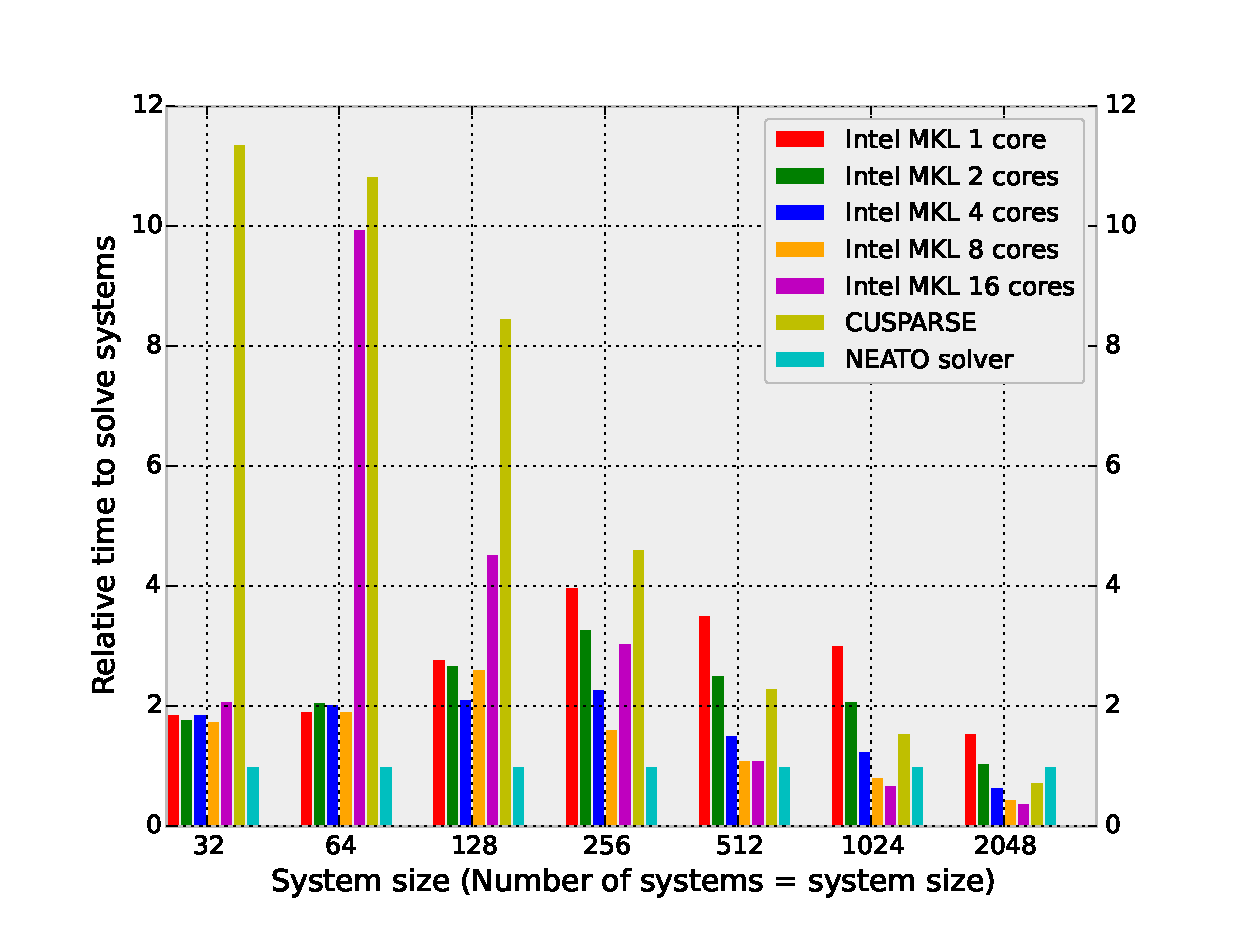
\includegraphics[width=180px]{img/bench-2d.eps}
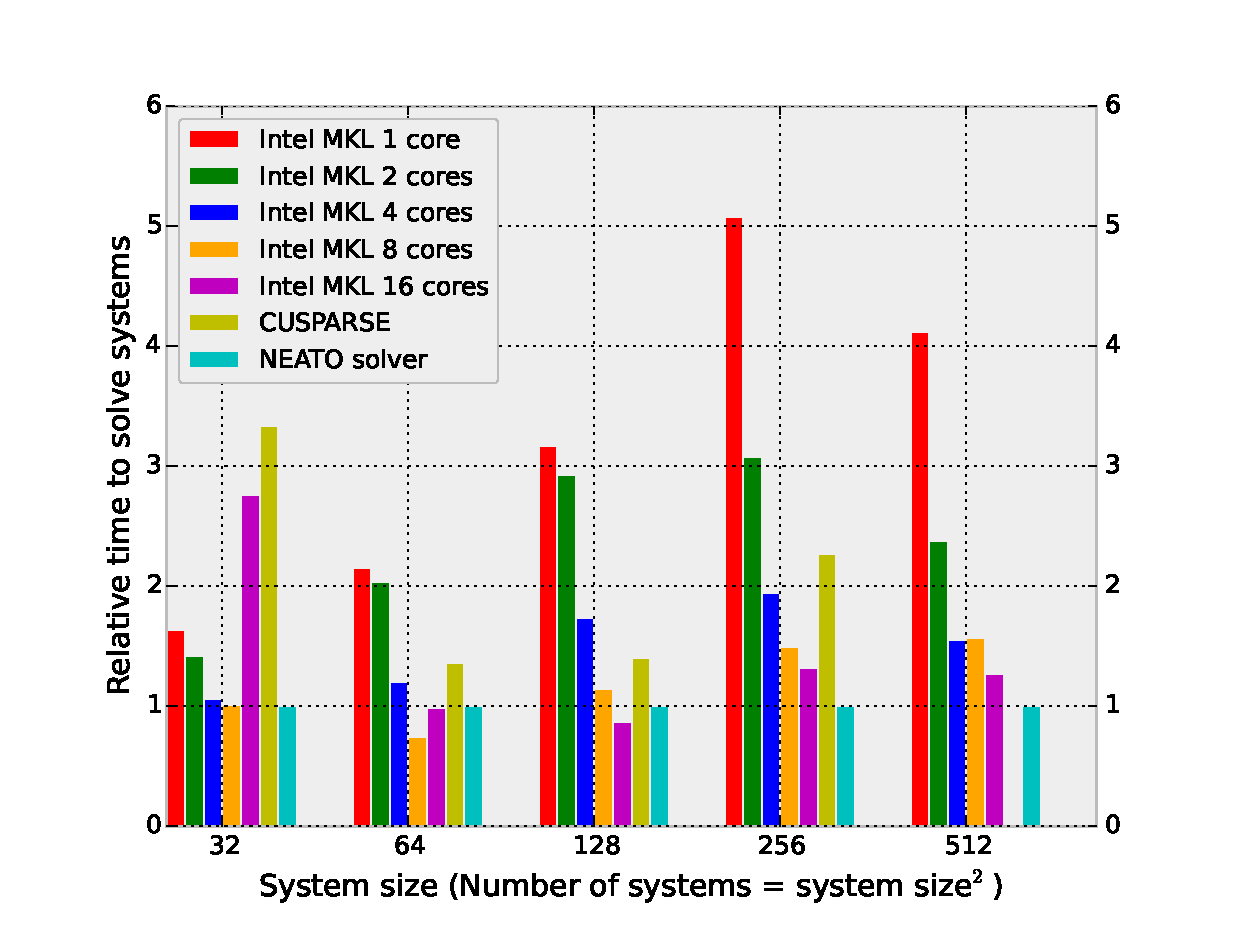
\includegraphics[width=180px]{img/bench-3d.eps}
\end{center}
\end{frame}

\begin{frame}
\frametitle{Comparison with library solvers - timings}
Timings for various solvers:
\begin{table}
\resizebox{\textwidth}{!}{%
% Please add the following required packages to your document preamble:
% \usepackage{multirow}
\begin{tabular}{|l|l|l|l|l|l|l|}
\hline
\multirow{2}{*}              & \multirow{2}{*}{}        & \multicolumn{5}{c|}{Time to solve (ms)}                             \\ \cline{3-7}
\centering System size       & Number of systems        & MKL 1 core    & MKL 16 cores & CUSPARSE & NEATO (global) & NEATO (shared) \\ \hline
32                           & 32                       & 0.045         & 0.05         & 0.273    & 0.201          & 0.024          \\ \hline
64                           & 64                       & 0.048         & 0.249        & 0.271    & 0.247          & 0.025          \\ \hline
128                          & 128                      & 0.089         & 0.145        & 0.271    & 0.284          & 0.032          \\ \hline
256                          & 256                      & 0.263         & 0.202        & 0.305    & 0.326          & 0.066          \\ \hline
512                          & 512                      & 0.959         & 0.299        & 0.629    & 0.403          & 0.272          \\ \hline
1024                         & 1024                     & 3.775         & 0.864        & 1.939    & 1.375          & 1.252          \\ \hline
2048                         & 2048                     & 16.272        & 4.111        & 7.607    & 5.811          & 10.407         \\ \hline
32                           & 1024                     & 0.152         & 0.257        & 0.31     & 0.207          & 0.092          \\ \hline
64                           & 4096                     & 0.879         & 0.403        & 0.556    & 0.751          & 0.409          \\ \hline
128                          & 16384                    & 7.052         & 1.931        & 3.128    & 3.669          & 2.225          \\ \hline
256                          & 65536                    & 63.858        & 17.61        & 28.495   & 21.148         & 12.565         \\ \hline
512                          & 262144                   & 515.792       & 159.394      &          & 145.34         & 125.311        \\ \hline 
\end{tabular}

}
\end{table}
\end{frame}

\begin{frame}
\frametitle{Note on speedups}
\begin{itemize}
\item Faster than CUSPARSE in almost all cases
\item Comparing against 8 CPU cores,
    speedups over MKL in the range 1-2x
\item Solving the tridiagonal systems
    \emph{least amenable to efficient parallel solution}
\item Objective is to keep the problem on the GPU
\item Multicore CPU performance flattens out
\end{itemize}
\end{frame}

\begin{frame}{Compact finite difference evaluation}
\footnotesize
\begin{block}{Benchmark details}
\begin{itemize}
\item Compact finite difference evaluation in 3-D for a function $f(x, y, z)$
\item Problem size up to $2048^3$ on up to 64 GPUs and 512 CPU cores
\item Tests performed on Palmetto cluster (Infiniband interconnect)
\end{itemize}
\end{block}
\end{frame}

\begin{frame}
\frametitle{Compact finite difference evaluation - profiling}
\begin{columns}
\begin{column}{0.5\textwidth}
\begin{itemize}
\item Problem sizes: $1024^3$ and $2048^3$ on 64 GPUs
\item Most time spent on solving tridiagonal systems
    \begin{itemize}
        \item Justifies optimization effort
    \end{itemize}
\item Significant portion of time spent on
    data permutation
    \begin{itemize}
        \item na\"{\i}ve implementation
    \end{itemize}
\end{itemize}
\end{column}
\begin{column}{0.5\textwidth}
\centering
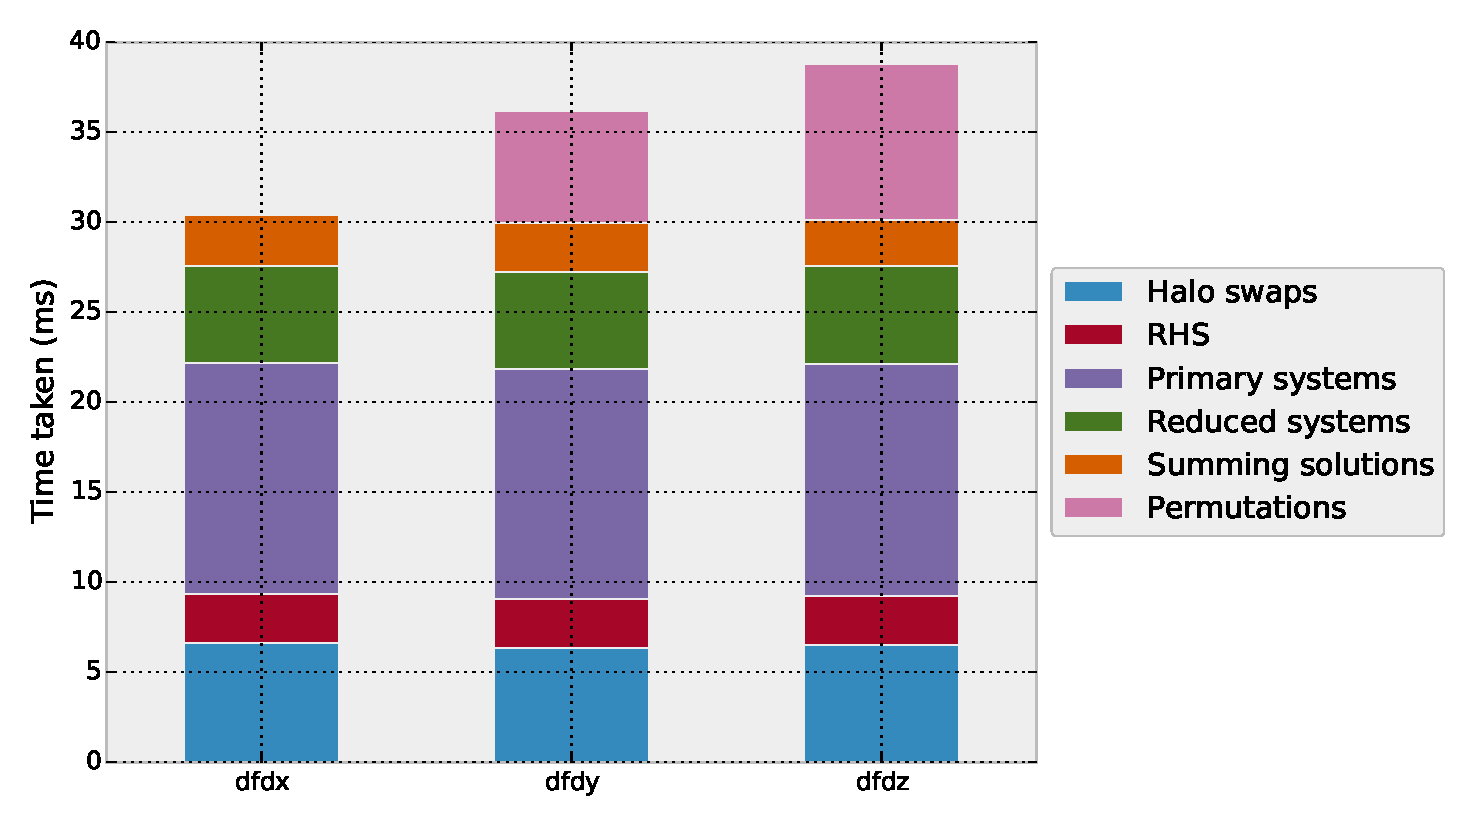
\includegraphics[width=170px]{img/profiling-1024-64.eps}

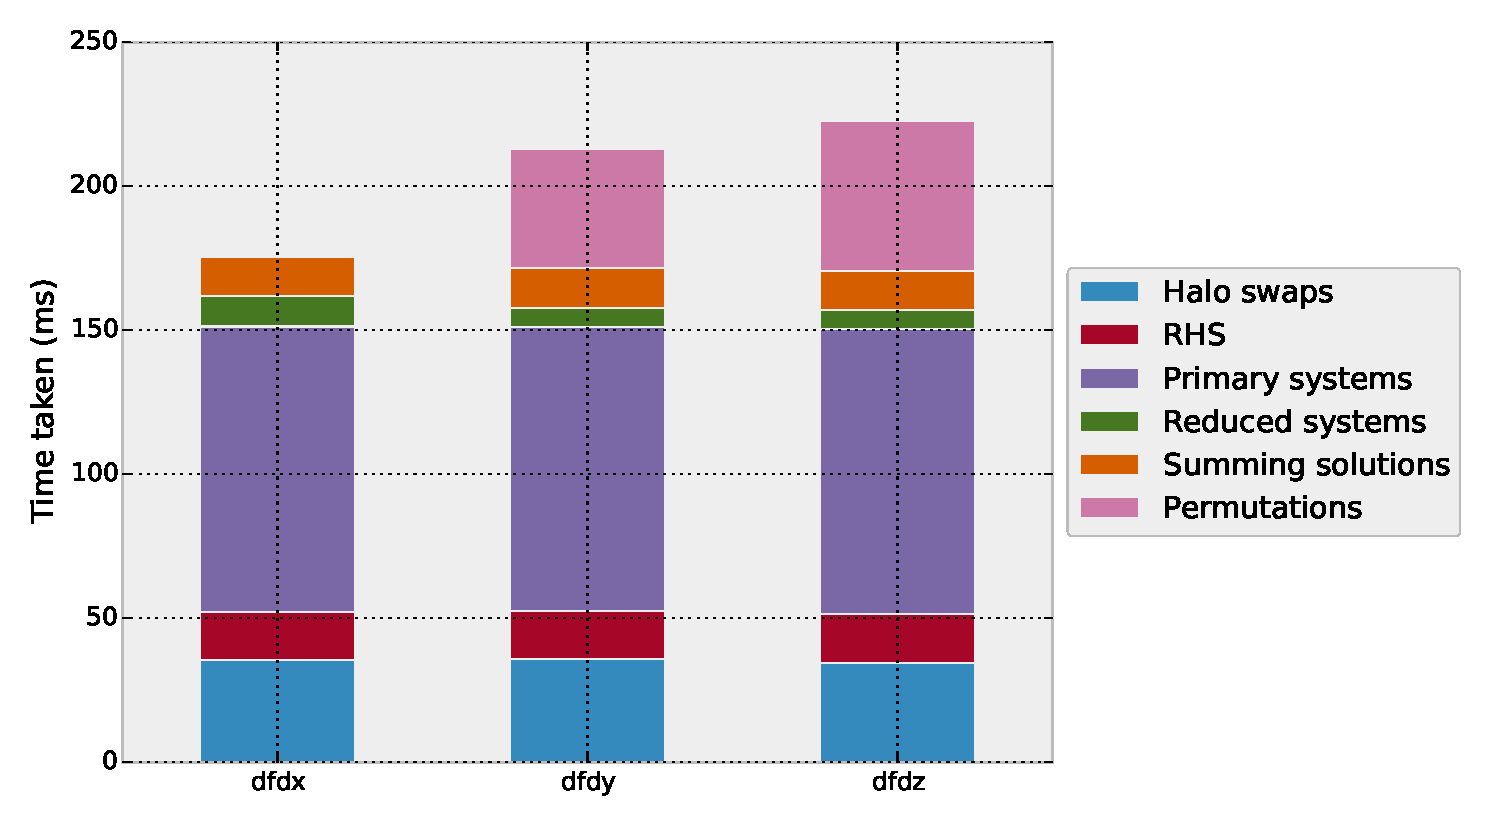
\includegraphics[width=170px]{img/profiling-2048-64.eps}
\end{column}
\end{columns}
\end{frame}

\begin{frame}
\frametitle{Compact finite difference evaluation - strong scaling}
\centering
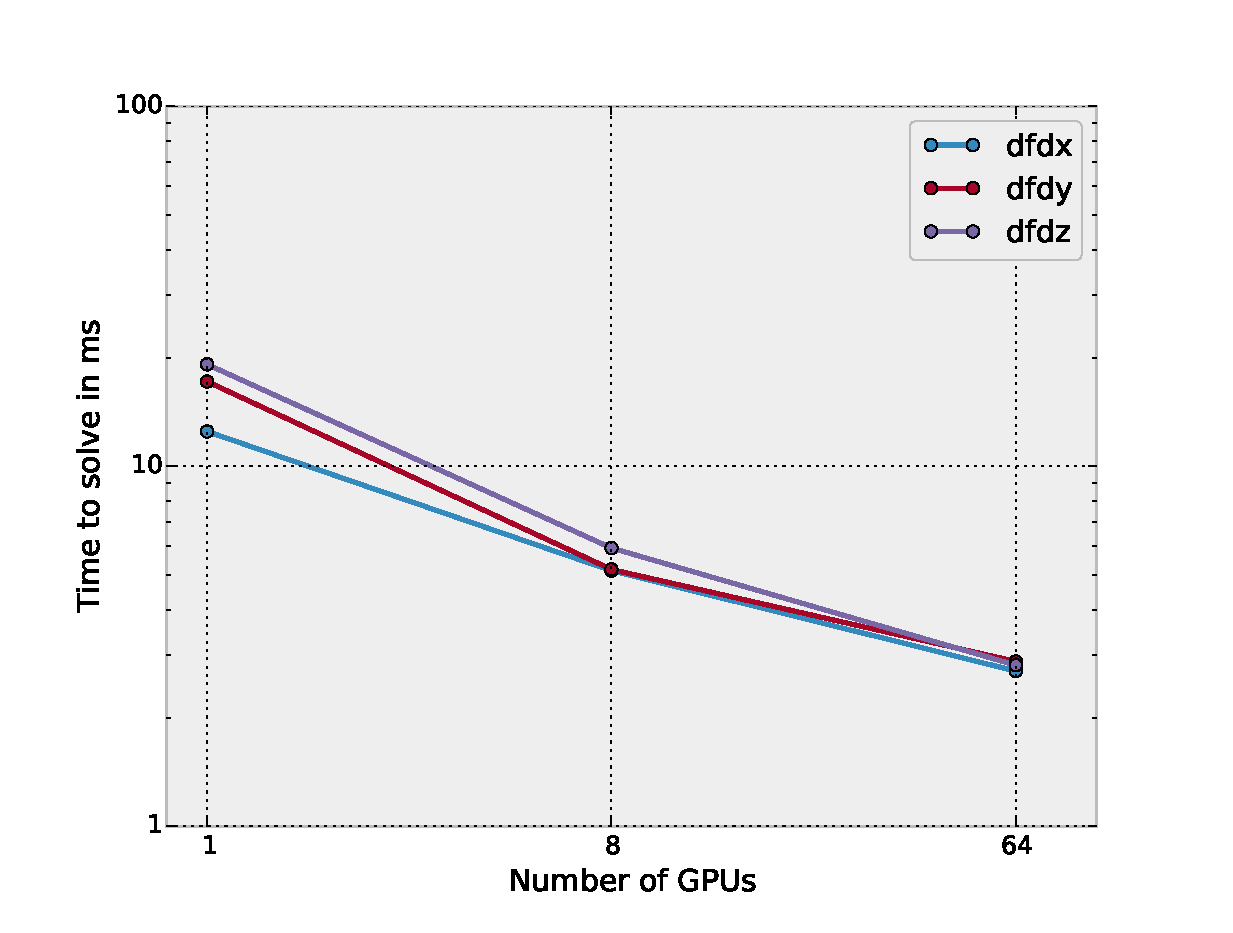
\includegraphics[width=180px]{img/strong-scaling-256.eps}
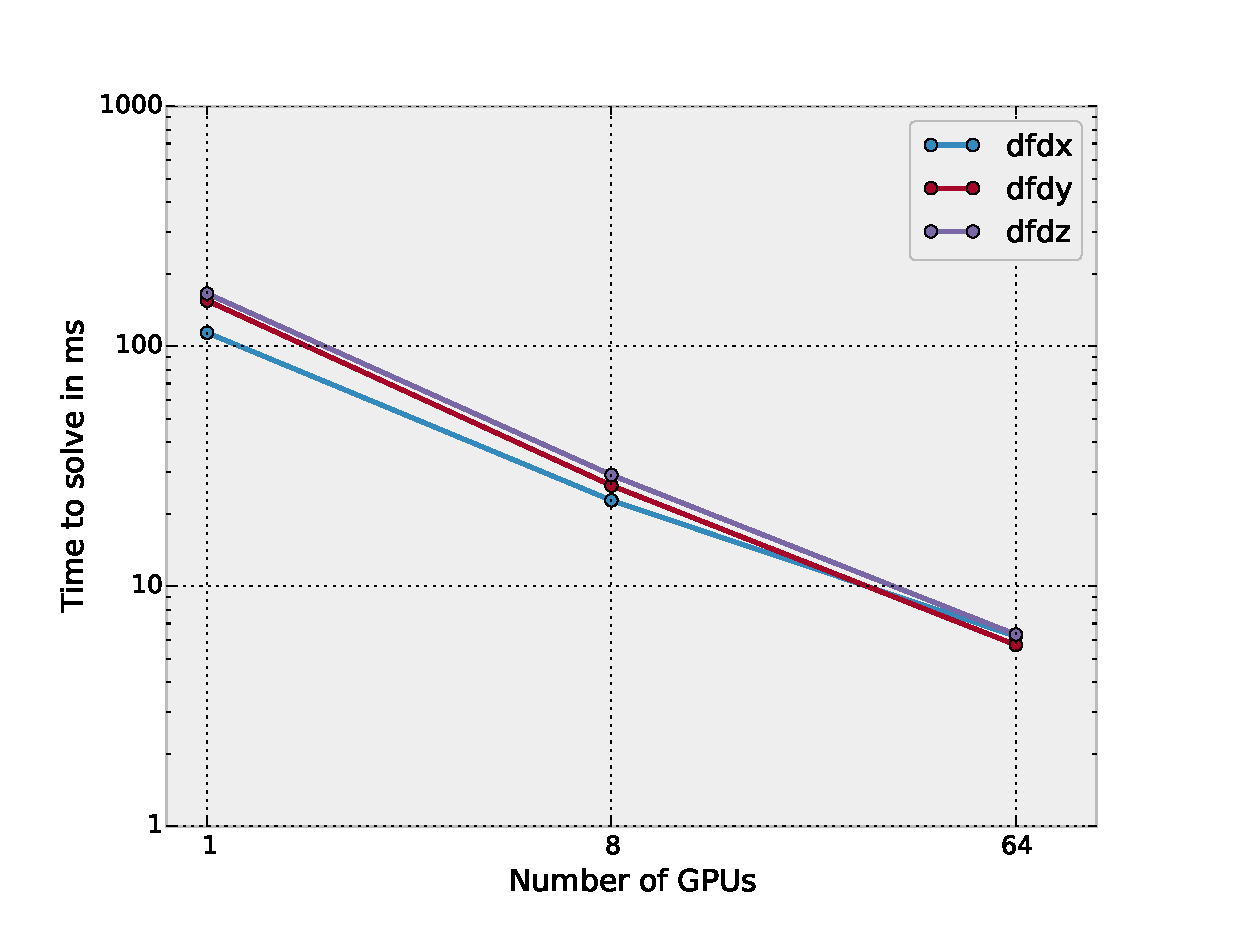
\includegraphics[width=180px]{img/strong-scaling-512.eps}

Problem sizes: $256^3$ and $512^3$
\end{frame}

\begin{frame}
\frametitle{Compact finite difference evaluation - weak scaling}
\centering
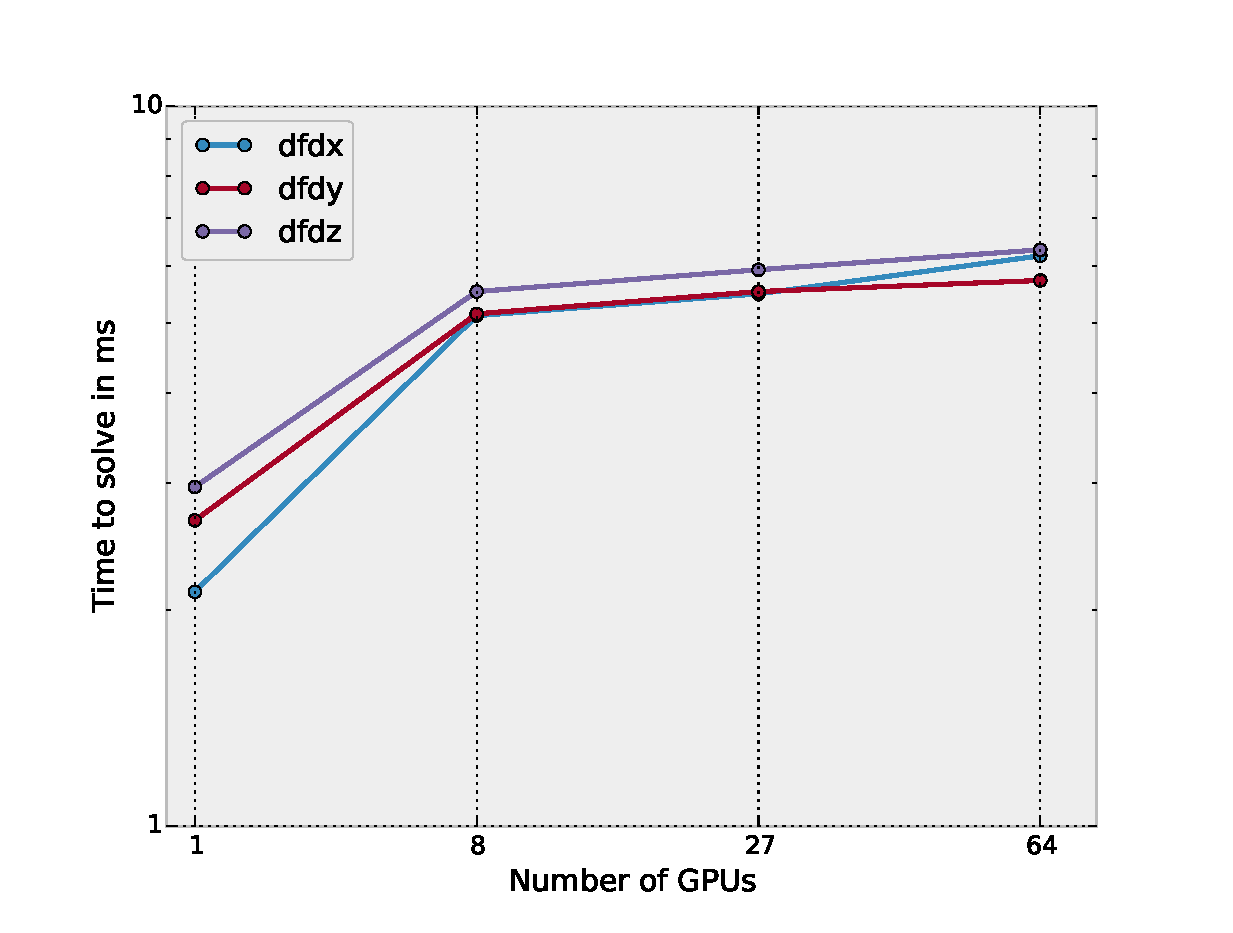
\includegraphics[width=180px]{img/weak-scaling-128.eps}
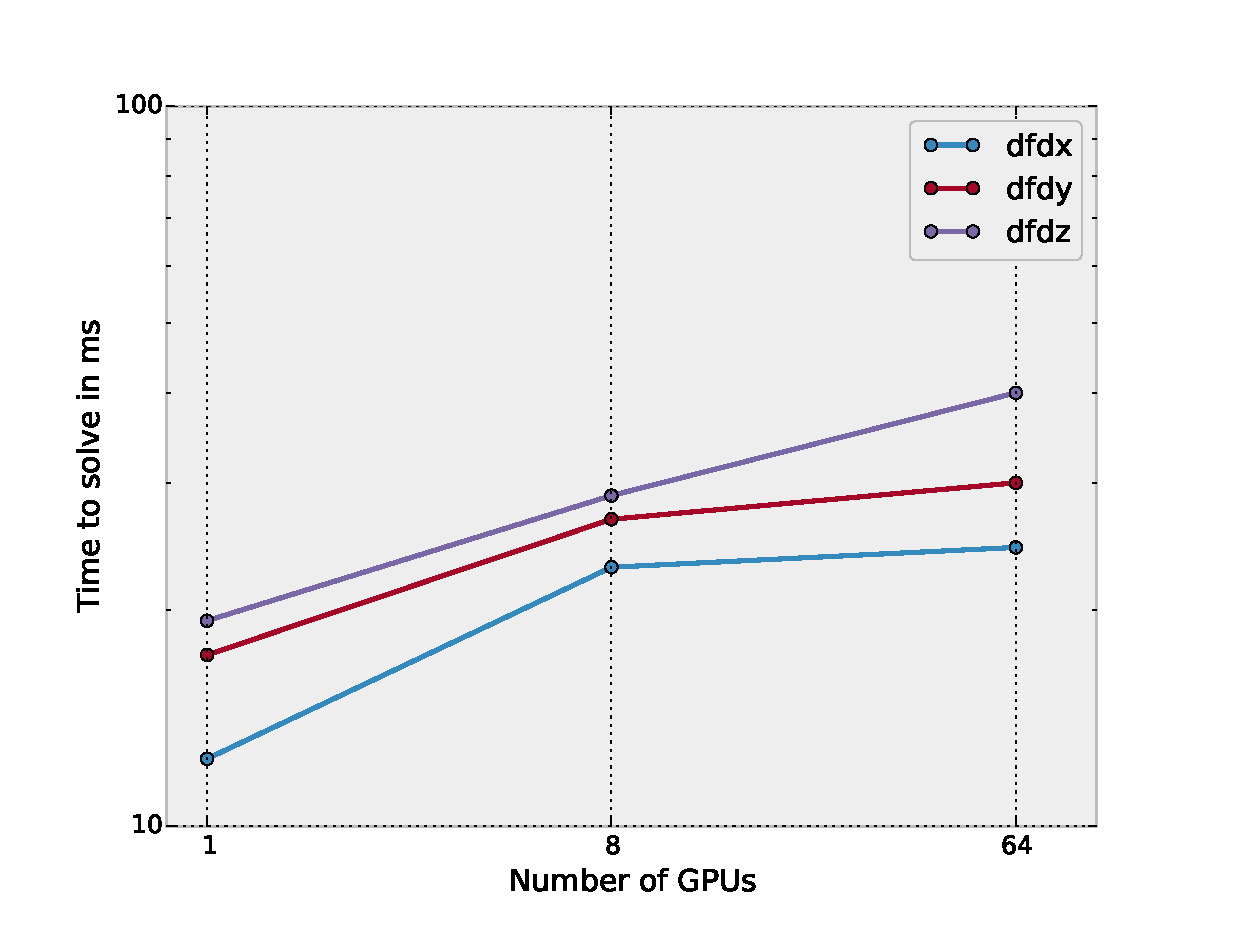
\includegraphics[width=180px]{img/weak-scaling-256.eps}

Problem sizes: $128^3$ and $256^3$ \emph{per process}
\end{frame}

\begin{frame}
\frametitle{Comparison with CPU-only approach}
\begin{columns}
\begin{column}{0.5\textwidth}
\begin{itemize}
\item Reference implementation: CFDNS
    (Los Alamos National Lab)
\item Uses LU algorithm
\item Parallelized among individual cores
\item Maintain a ratio of 8 CPU cores : 1 GPU for comparison
\end{itemize}
\end{column}
\begin{column}{0.5\textwidth}
\centering
\begin{table}
\resizebox{0.75\textwidth}{!}{%
\centering
\begin{tabular}{|l|l|l|l|l|l|l|}
\hline
\multirow{2}{*}{Size} & \multicolumn{3}{c|}{Ref. impl, \#CPU cores} & \multicolumn{3}{c|}{NEATO-based, \#GPUs} \\ \cline{2-7}
         & 8         & 64        & 512      & 1       & 8       & 64      \\ \hline
$256^3$  & 79.5      & 20.8      & 11.1     & 19.9    & 5.17    & 2.79    \\ \hline
$512^3$  & 556.8     & 146.5     & 29.2     & 164.5   & 23.24   & 5.62    \\ \hline
$1024^3$ & 5188      & 1092      & 223.7    & -       & 174.9   & 24.49   \\ \hline
$2048^3$ & -         & -         & 1741     & -       & -       & 297.07  \\ \hline
\end{tabular}

}
\end{table}

\includegraphics[width=140px]{img/compact-refimpl-speedups.eps}
\end{column}
\end{columns}
\end{frame}

\begin{frame}
\frametitle{Conclusions and future work}
\begin{itemize}
    \item Tridiagonal solver performance
        is key in compact finite difference evaluation
    \item Simple matrix structure can be exploited
        in the cyclic reduction algorithm
    \item Substantial speedups can be achieved
        over CPU
    \item Applicability to other algorithms: PCR, CR+PCR
    \item Integration into current DNS code
    \item Strategies for MIC architecures
\end{itemize}
\end{frame}

\begin{frame}
    Thank you    
\end{frame}

